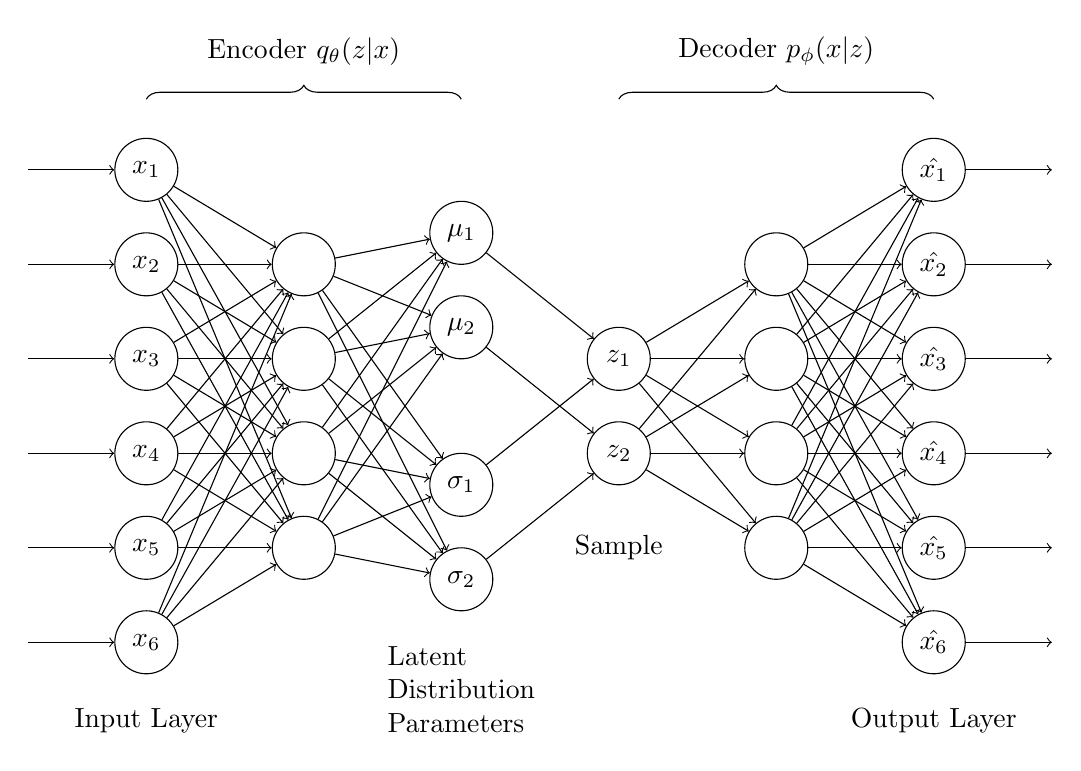
\begin{tikzpicture}
    \tikzstyle{place}=[circle, draw=black, minimum size = 8mm]
    
    % Input
    \foreach \x in {1,...,6}
        \draw node at (0, -\x*1.2) [place] (first_\x) {$x_\x$};
    
    % Hidden 1
    \foreach \x in {1,...,4}
        \node at (2, -1.2 -\x*1.2) [place] (second_\x){};

    % Mu
    \foreach \x in {1,...,2}
        \node at (4, -0.8 -\x*1.2) [place] (mu_\x){$\mu_\x$};

    \foreach \x in {1,...,2}
        \node at (4, -4 -\x*1.2) [place] (logvar_\x){$\sigma_\x$};

    \foreach \x in {1,...,2}
        \draw node at (6, -2.4 -\x*1.2) [place] (sample_\x){$z_\x$};

    % Hidden 2
    \foreach \x in {1,...,4}
        \node at (8, -1.2 -\x*1.2) [place] (fourth_\x){};
    
    % Output
    \foreach \x in {1,...,6}
        \draw node at (10, -\x*1.2) [place] (fifth_\x) {$\hat{x_\x}$};
        
    \foreach \i in {1,...,6}
        \draw [->] (-1.5, -\i*1.2) to (first_\i);

    \foreach \i in {1,...,6}
        \foreach \j in {1,...,4}
        \draw [->] (first_\i) to (second_\j);

    \foreach \i in {1,...,4}
        \foreach \j in {1,...,2}
            \draw [->] (second_\i) to (mu_\j);
    \foreach \i in {1,...,4}
        \foreach \j in {1,...,2}
        \draw [->] (second_\i) to (logvar_\j);

    \foreach \i in {1,...,2}
        \draw [->] (logvar_\i) to (sample_\i);
    
    \foreach \i in {1,...,2}
        \draw [->] (mu_\i) to (sample_\i);

    \foreach \i in {1,...,2}
        \foreach \j in {1,...,4}
        \draw [->] (sample_\i) to (fourth_\j);
    
    \foreach \i in {1,...,4}
        \foreach \j in {1,...,6}
        \draw [->] (fourth_\i) to (fifth_\j);

    \foreach \i in {1,...,6}
        \draw [->] (fifth_\i) to (11.5, -\i*1.2);

    \draw [decorate,decoration={brace,amplitude=5pt,raise=-2ex}]
        (0,0) -- (4,0) node[above,midway]{Encoder $q_\theta(z|x)$};
    \draw [decorate,decoration={brace,amplitude=5pt,raise=-2ex}]
        (6,0) -- (10,0) node[above,midway]{Decoder $p_\phi(x|z)$};
    
    % Text
    \node at (0, -8.2) [black, ] {Input Layer};
    \node at (4, -7.8) [black, align=left] {Latent \\ Distribution\\ Parameters};
    \node at (6, -6) [black, ] {Sample};
    \node at (10, -8.2) [black, ] {Output Layer};
\end{tikzpicture}